És important tenir una planificació de tasques en els projectes grans, per tal de poder decidir aproximadament el temps a dedicar a cada secció del projecte.
Encara que no es segueixi al peu de la lletra serveix com a referència per la direcció del projecte.
\\ \\
L'objectiu inicial del projecte era acabar-lo i presentar-lo en la convocatòria de Septembre del 2019, però degut al incompliment dels requisits pel lliurament i presentació del treball l'objectiu va passar a ser el Septembre del 2020.
És per això que presentem dues planificacions temporals, una feta amb l'objectiu de presentar el Septembre del 2019, i una altre feta a dia 1 de Septembre del 2019 amb objectiu de presentar al cap d'un any.

\section{Planificació original}

\begin{figure}[H]
  \centering
  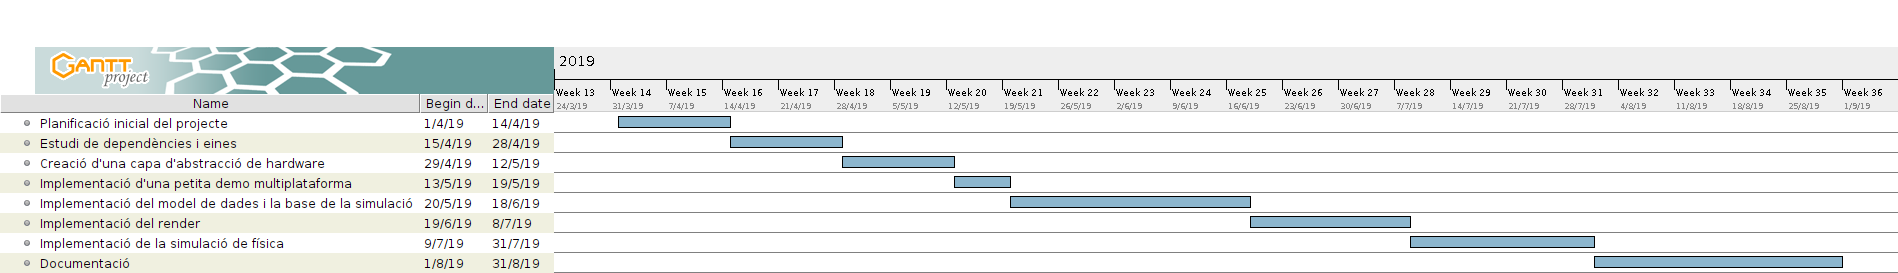
\includegraphics[angle=90,origin=c,scale=0.35]{img/planificacioOG}
  \caption{Diagrama de la planificació original}
\end{figure}
\section{Planificació final}
\begin{figure}[H]
  \centering
  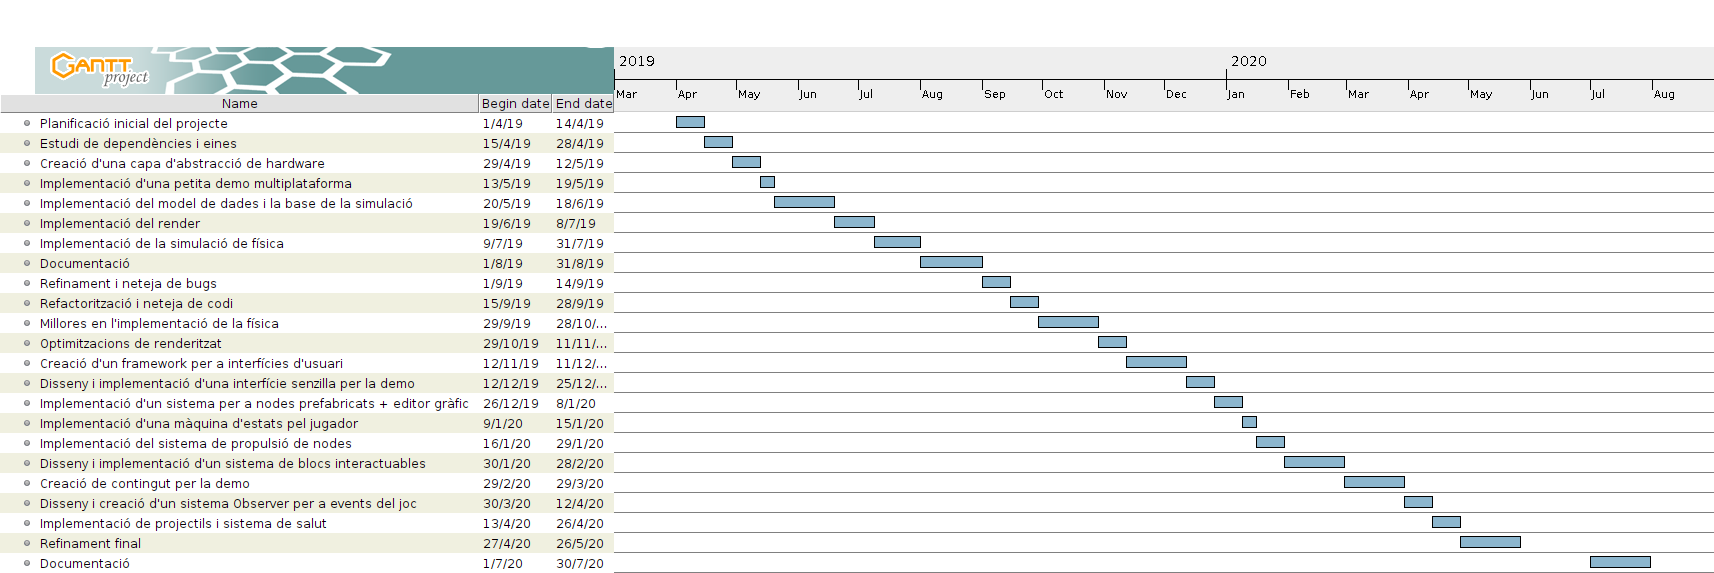
\includegraphics[angle=90,origin=c,scale=0.4]{img/novaPlanificacio}
  \caption{Diagrama de la planificació final}
\end{figure}

